% Why an evidence gap is not enough. The two points are the
% counterexample of Appendix B.4 (default weights, conf 0.5, cs 1, ca 1, HIGH):
%   correct:   ev 0.90, rec 0 -> 0.35*0.90 + 0.20*0.5 + 0.25 + 0    + 0.15 = 0.815
%   incorrect: ev 0.80, rec 1 -> 0.35*0.80 + 0.20*0.5 + 0.25 + 0.05 + 0.15 = 0.830
% Deadband: scores within 0.05 of the top score 0.830, i.e. [0.780, 0.830].
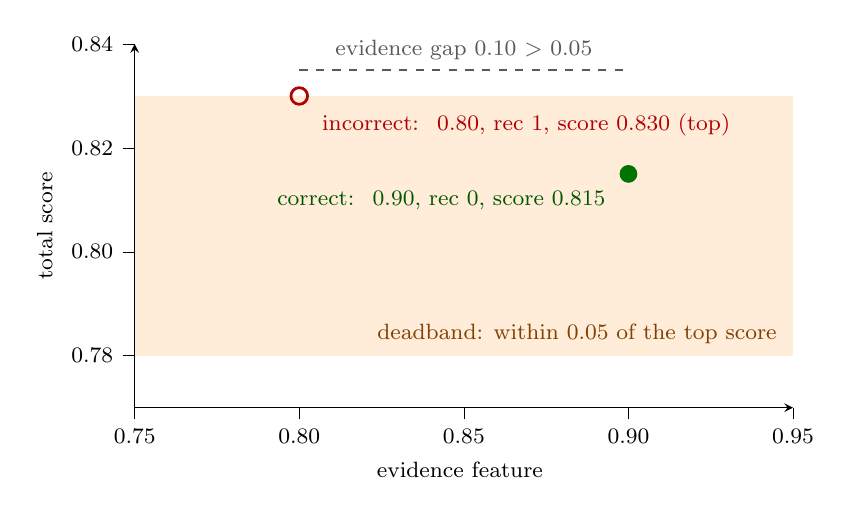
\begin{tikzpicture}
  \begin{axis}[
      width=0.82\linewidth, height=6.2cm,
      xmin=0.75, xmax=0.95, ymin=0.77, ymax=0.84,
      xtick={0.75,0.80,0.85,0.90,0.95},
      ytick={0.78,0.80,0.82,0.84},
      xticklabel style={/pgf/number format/.cd,fixed,fixed zerofill,precision=2},
      yticklabel style={/pgf/number format/.cd,fixed,fixed zerofill,precision=2},
      xlabel={evidence feature $\ev$}, ylabel={total score},
      axis lines=left, tick align=outside, tick style={black},
      font=\footnotesize, clip=false]
    \fill[orange!15] (axis cs:0.75,0.780) rectangle (axis cs:0.95,0.830);
    \node[anchor=south east,text=orange!50!black] at (axis cs:0.948,0.7805)
      {deadband: within 0.05 of the top score};
    \draw[dashed,black!65] (axis cs:0.80,0.8350) -- (axis cs:0.90,0.8350)
      node[midway,above,text=black!65] {evidence gap 0.10 $>$ 0.05};
    \addplot[only marks,mark=o,mark size=3pt,draw=red!70!black,line width=1pt]
      coordinates {(0.80,0.830)};
    \addplot[only marks,mark=*,mark size=3pt,color=green!45!black]
      coordinates {(0.90,0.815)};
    \node[anchor=north west,text=red!70!black] at (axis cs:0.804,0.8285)
      {incorrect: $\ev$ 0.80, rec 1, score 0.830 (top)};
    \node[anchor=north east,text=green!35!black] at (axis cs:0.896,0.8135)
      {correct: $\ev$ 0.90, rec 0, score 0.815};
  \end{axis}
\end{tikzpicture}
